\chapter {Planning}

\section {Chemical Ideas}

In this section.

	\subsection{Rate of Reactions}




	\subsection{pH}

The pH scale is composed of two extremes that describes a chemical property about the substance being tested, these extremes are called acids and bases. Mixing acids and bases together will induce a neutralisation reaction which can cancel out their extreme effects. A substance which is neither acidic nor basic is called a neutral substance. The pH scale ranges from 0 to 14, with 0 being as acidic as possible and 14 being as basic as possible. Neutral has a corresponding pH of 7 and therefore anything below 7 is acidic and anything above 7 is basic. The pH scale is illistrated below.


\begin{figure}[H]
    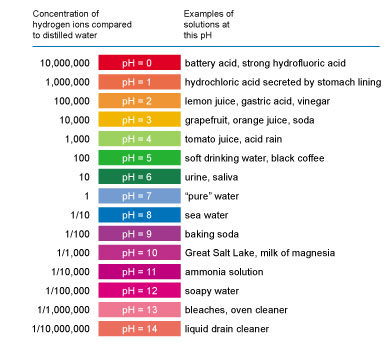
\includegraphics[width=\textwidth]{./Planning/Images/pHScale.jpg}
    \caption{The pH scale} \label{fig:pH Scale}
\end{figure}

The pH scale is a man made scale which is used to measure the concentration of hydrogen ions, each concentration is given a corresponding place on the scale (pH). pH is mathematically defined as the negative logarithm of the hydrogen ion concentration. As a result of this we can determine that the pH scale is logarithmic, therefore each value above/below the neutral value (7) is ten times more basic/acidic respectively. For example pH 6 is ten times as acidic as pH 7  and pH 5 is one hundred times as acidic than pH 7. The mathematical equation for working out pH is illistrated below.

\begin{itemize}
\item pH = - log [H\^+]
\end{itemize}

There are many indicators used to find out the pH of substances. A table of common indicators with their properties are displayed in the table below.

\begin{figure}[H]
    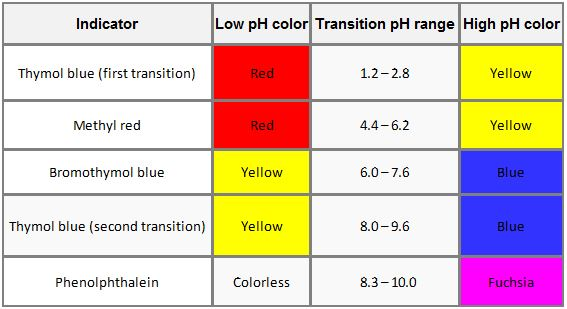
\includegraphics[width=\textwidth]{./Planning/Images/Indicators.jpg}
    \caption{List of pH Indicators} \label{fig:pH Indicators}
\end{figure}

Universal indicator contains all of the chemicals above, all mixed into a single solution or into universal indicator paper. This allows for a continuous color change from about pH 2 to pH 10. Visual comparison of the colour of the universal indicator and a standard colour chart give a rough reading of the pH of the substance being measured, usually to the nearest whole number. 


	\subsection{Acids}

The Brønsted–Lowry theory defines an acid as a proton (H+) donor. 

-Weak/strong (organic/inorganic) (dissociation)
-Low conc/High conc



	\subsection{Catalysts}




	\subsection{Factors that affect Rate of Reaction}



	\subsection{Enthalpy Level Diagrams}	



	\subsection{Methods of Finding Rates}



		\subsubsection{Justification of Chosen Method}

I will be 



	\subsection{How the Rate of Reaction is Determined Experimentally}



	\subsection{Rate Equations}



	\subsection{Orders of Reactions}



	\subsection{Transition Metal Catalysts}



	\subsection{D-Orbitals}



	\subsection{Complexes and their Properties}


\section{Inventory}

	\subsection{Equipment List}
\begin{itemize}
\item 250 cm3 conical flask.
\item Bung fitted to a glass tube.
\item Burette.
\end{itemize}

	\subsection{Chemical List}
\begin{itemize}
\item Distilled Water.
\item 0.20 moldm-3 Copper Sulfate (aq).
\item 1.0 moldm-3 Sulfuric Acid (aq).
\item Granulated Zinc (s).
\item Mixture of Different Catalysts.
\end{itemize}



\section{Methods}

	\subsection{Chosen Method}

\textbf{Setting Up}

\begin{enumerate}
\item Fill the Burette with distilled water.
\item Fit the bung (fitted with glass tube) into the conical flask.
\item Fit the inverted Burette to the end of the glass tube.
\end{enumerate}

\textbf{Carrying out the Experiment}

\begin{enumerate}
\item Remove the bung from the conical flask and pour 30 cm3 of distilled water and 10 cm3 of sulfuric acid into the conical flask.
\item Weigh out 1.0 g of granulated zinc.
\item Add the measured 1.0 g of granulated zinc to the conical flask.
\item Place the bung back in the conical flask.
\item Record the volume of hydrogen produced in cm3 every 30 seconds for 5 minutes from the burette markings to 1 decimal place.
\item Repeat the experiment but use 30cm3 of copper sulfate instead of distilled water.
\end{enumerate} 

\textbf{Interpreting the Data (as discussed before)}

\begin{enumerate}
\item Plot a graph of the volume of hydrogen against time.
\item From the graph draw a tangent to the line at the initial point.
\item Calculate the gradient of the tangent by using the equation: 
\item The gradient is equal to the rate of reaction.
\end{enumerate}



	\subsection{Justification of Chosen Method}

In addition to the method discussed above, there are two other methods which would allow me to carry out my experiment:
\begin{itemize}
\item The Gas Syringe Method
\item The Mass Change Method 
\end{itemize}

Below, the methods are explained:

\textbf{Gas Syringe Method}



Setting up involves a similar set up to my chosen method, but the gas syringe replaces the burette. This is shown below:
\begin{figure}[H]
    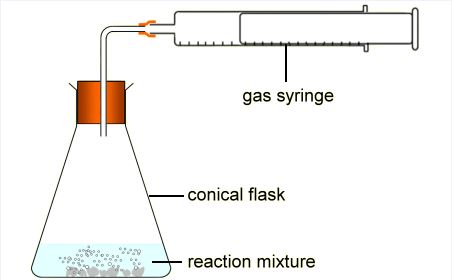
\includegraphics[width=\textwidth]{./Planning/Images/GasSyringe.jpg}
    \caption{Gas Syringe Equipment} \label{fig:Gas Syringe}
\end{figure}

Carrying out the method is precisely the same as my chosen method except a reading is taken from the gas syringe instead of the burette. This is precisely the reason I have chosen to not use this method. The gas syringes available to me have graduations every 1ml, whereas the burrettes available to me have graduations every 0.1ml. Therefore the accuracy of my readings will be greater using the burette method and consequently I have chosen the burette method ovet the gas syring method. 

\textbf{Mass Change Method}

Setting up this method involves:
\begin{itemize}
\item Balance (reading to 0.01 g)
\item Conical Flask
\item Cotton Wool
\end{itemize}

Carrying out this method involves:

\begin{enumerate}
\item Zero the Balance.
\item Pour 30 cm3 of distilled water and 10 cm3 of sulfuric acid into the conical flask.
\item Take note of the Balance value + 1.0 g
\item Weigh out 1.0 g of granulated zinc.
\item Add the measured 1.0 g of granulated zinc to the conical flask.
\item Place the cotton wool in the conical flask to stop acid 'spray' excaping.
\item Record the loss in mass in grams every 30 seconds for 5 minutes to 2 decimal places.
\item Repeat the experiment but use 30cm3 of copper sulfate instead of distilled water.
\end{enumerate} 

I have chosen not to carry out this method as the balance will be a lot more sensitive to the environment and there will be room for a lot more human error. For example, left over residue could land on the scales and scew the results during the experiment. 


\begin{landscape}

\section{Risk Assessment}

\begin{center}
\begin{longtable}{|p{1.5cm}|p{1.5cm}|p{3cm}|p{3cm}|p{3cm}|p{3cm}|p{2cm}|}
    \hline
 \textbf{Name of Chemical} & \textbf{Source of Information} & \textbf{Hazards} & \textbf{Risks} & \textbf{Control Measures} & \textbf{Disposal Method} & \textbf{Emergency Procedures} \\ \hline

Copper Sulfate (aq) &
CLEAPSS Hazcards &
\begin{itemize}
\item Harmful
\item Dangerous for the Environment \end{itemize} &
\begin{itemize}
\item Harmful if swallowed
\item Irritating to eyes and skin \end{itemize} &
\begin{itemize}
\item Do not put near mouth
\item Use gloves
\item Use goggles
\item Keep away from water, unless intended. \end{itemize} & 
Dissolve 64 g in 1 litre of water before pouring the solution down a foulwater drain. This disposal procedure should be kept to a minimum. &
Seek medical attention. Wash contaminated area. \\ \hline

Hydrated Copper Sulfate (s) &
CLEAPSS Hazcards &
\begin{itemize}
\item Harmful
\item Dangerous for the Environment \end{itemize} &
\begin{itemize}
\item Harmful if swallowed
\item Irritating to eyes and skin \end{itemize} &
\begin{itemize}
\item Do not put near mouth
\item Use gloves
\item Use goggles
\item Label: Harmful, if above 1moldm-3 \end{itemize} &
Crystals may be used for solutions. Dilute to less than 0.4 mol dm-3 or dissolve 100 g in 1 litre of water before pouring the solution down a foul-water drain. This disposal procedure should be kept to a minimum . &
Seek medical attention. Wash contaminated area. \\ \hline



Sulfuric Acid (aq) &
CLEAPSS Hazcards &
\begin{itemize}
\item Corrosive
\item Irritant \end{itemize} &
Causes serious burns & 
\begin{itemize}
\item Label: Irritant, if above 0.5 moldm-3
\item Label: Corrosive, if above 1.5 moldm-3
\item Wear gloves
\item Wear goggles \end{itemize} &
Add slowly no more than 10 cm3 of concentrated sulfuric(VI) acid to 1 litre of 1 mol dm-3 sodium carbonate solution (containing indicator) which should be constantly stirred. Let the mixture cool (or add ice), before adding more acid. Pour the solution down a foul-water drain. & 
Remove contaminated clothing and quickly wipe as much liquid as possible off the skin with a dry cloth before drenching the area with a large excess of water. If a large area is affected or blistering occurs, seek medical attention. \\ \hline

Granulated Zinc (s) &
CLEAPSS Hazcards &
\begin{itemize}
\item Low Hazard \end{itemize} &
N/A &
Place in normal refuse &
N/A &
N/A \\ \hline

\end{longtable}
\label{tab:Risk Assessment Table}

\end{center}


\end{landscape}



